%!\subsection{Quantitative complexity Analysis}
%    \label{subsec:ComplexityImageAnalysis}
%    %!\subsection{Quantitative complexity Analysis}
%    \label{subsec:ComplexityImageAnalysis}
%    %!\subsection{Quantitative complexity Analysis}
%    \label{subsec:ComplexityImageAnalysis}
%    %!\subsection{Quantitative complexity Analysis}
%    \label{subsec:ComplexityImageAnalysis}
%    \input{Text/ResultsImageComplexityAnalysisHistory.tex}

We have previously discussed the argument that the architectural evolution, throughout history, has been characterized by a continual interplay between simplicity and complexity.
This notion has been substantiated by our exploration of the theoretical definitions and varied approaches to facades and ornamentation within the context of prominent architectural styles and the perspectives of their eminent architects.

Our literature review has consistently pointed towards a prevailing trend in contemporary architecture, suggesting a resurgence of complexity in architectural design.
However, to ensure our findings are not purely subjective or biased towards this conclusion, we have conducted a quantitative analysis using the Computational Image Complexity Analysis (CICA) system.
This rigorous analysis method utilizes input images of the most iconic and representative buildings from various epochs and styles.

The results are visually depicted in Figure\ref{fig:HistoricalComplexityGraph}, where a discernible upward trendline towards complexity emerges, particularly noticeable since the late 20th century.

%% Figure of Complexity graph
     \begin{figure*}[!htb]
          \centering
          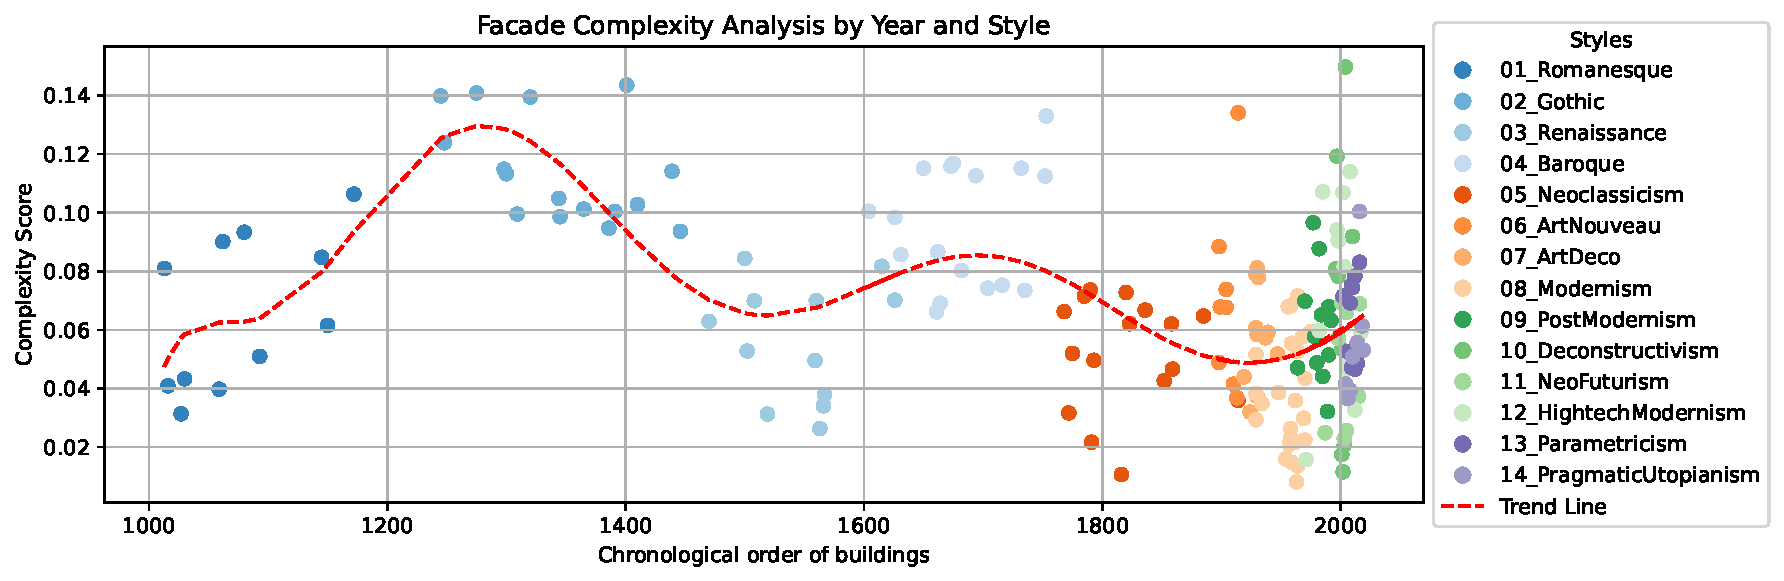
\includegraphics[width= \linewidth]{Graphs/complexitygraph}
          \caption{Scatter graph showcasing quantitative image complexity analysis scores for building images categorized by historical timeline and architectural style, with an overlaid trendline highlighting the evolving trend towards increased complexity.}
          \label{fig:HistoricalComplexityGraph}
     \end{figure*}










We have previously discussed the argument that the architectural evolution, throughout history, has been characterized by a continual interplay between simplicity and complexity.
This notion has been substantiated by our exploration of the theoretical definitions and varied approaches to facades and ornamentation within the context of prominent architectural styles and the perspectives of their eminent architects.

Our literature review has consistently pointed towards a prevailing trend in contemporary architecture, suggesting a resurgence of complexity in architectural design.
However, to ensure our findings are not purely subjective or biased towards this conclusion, we have conducted a quantitative analysis using the Computational Image Complexity Analysis (CICA) system.
This rigorous analysis method utilizes input images of the most iconic and representative buildings from various epochs and styles.

The results are visually depicted in Figure\ref{fig:HistoricalComplexityGraph}, where a discernible upward trendline towards complexity emerges, particularly noticeable since the late 20th century.

%% Figure of Complexity graph
     \begin{figure*}[!htb]
          \centering
          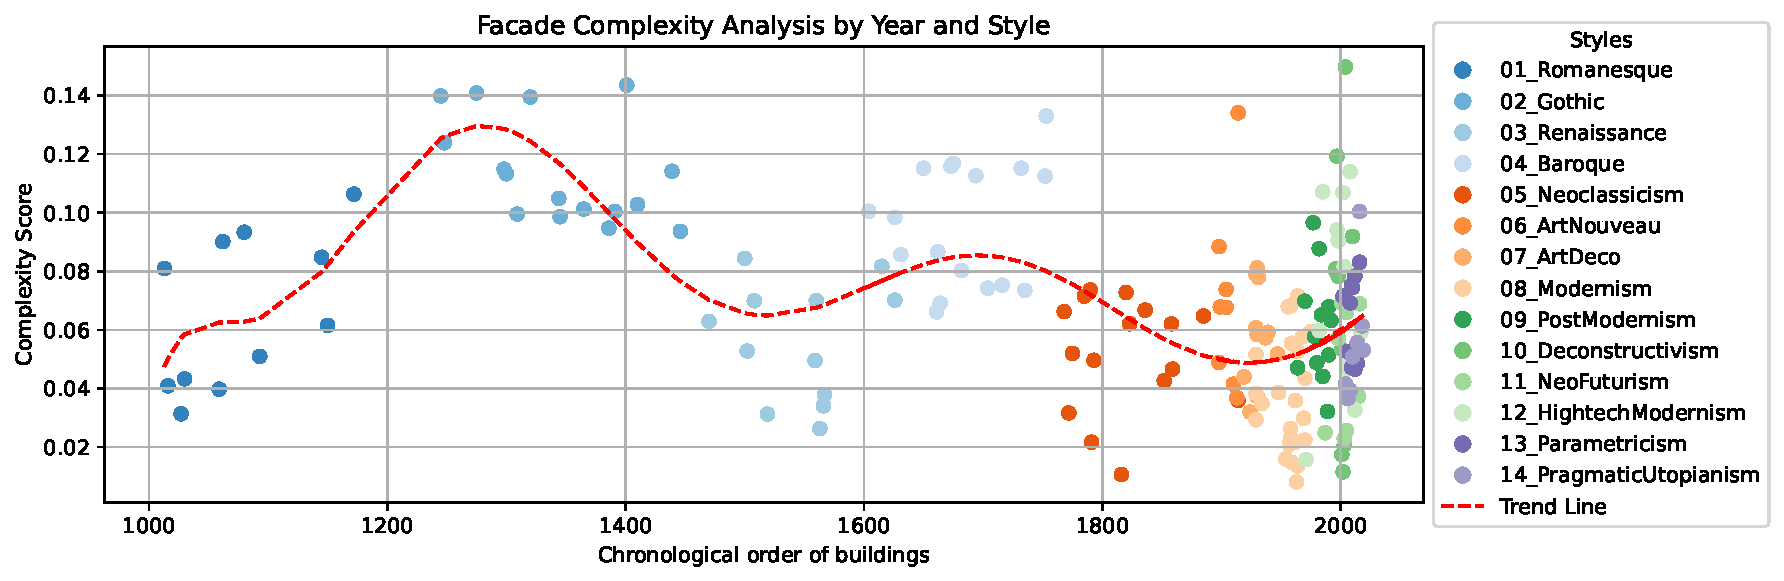
\includegraphics[width= \linewidth]{Graphs/complexitygraph}
          \caption{Scatter graph showcasing quantitative image complexity analysis scores for building images categorized by historical timeline and architectural style, with an overlaid trendline highlighting the evolving trend towards increased complexity.}
          \label{fig:HistoricalComplexityGraph}
     \end{figure*}










We have previously discussed the argument that the architectural evolution, throughout history, has been characterized by a continual interplay between simplicity and complexity.
This notion has been substantiated by our exploration of the theoretical definitions and varied approaches to facades and ornamentation within the context of prominent architectural styles and the perspectives of their eminent architects.

Our literature review has consistently pointed towards a prevailing trend in contemporary architecture, suggesting a resurgence of complexity in architectural design.
However, to ensure our findings are not purely subjective or biased towards this conclusion, we have conducted a quantitative analysis using the Computational Image Complexity Analysis (CICA) system.
This rigorous analysis method utilizes input images of the most iconic and representative buildings from various epochs and styles.

The results are visually depicted in Figure\ref{fig:HistoricalComplexityGraph}, where a discernible upward trendline towards complexity emerges, particularly noticeable since the late 20th century.

%% Figure of Complexity graph
     \begin{figure*}[!htb]
          \centering
          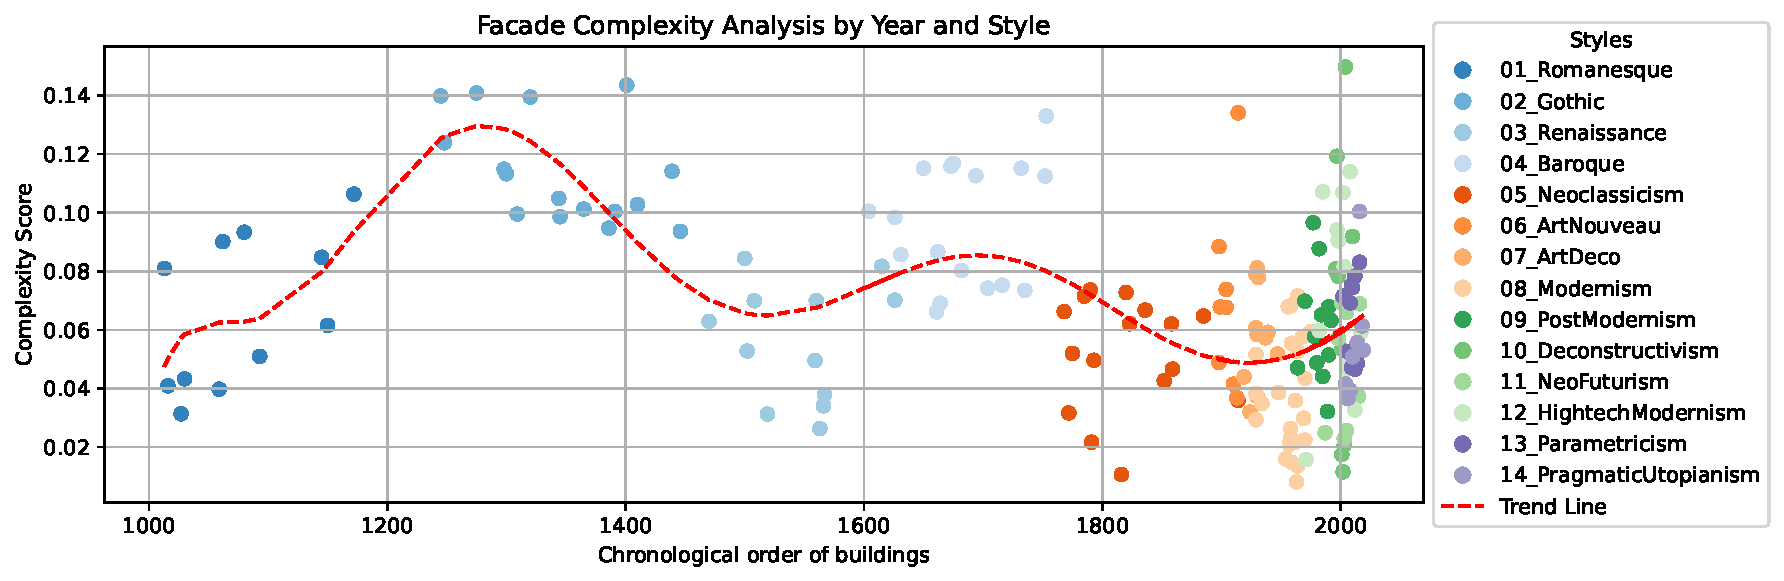
\includegraphics[width= \linewidth]{Graphs/complexitygraph}
          \caption{Scatter graph showcasing quantitative image complexity analysis scores for building images categorized by historical timeline and architectural style, with an overlaid trendline highlighting the evolving trend towards increased complexity.}
          \label{fig:HistoricalComplexityGraph}
     \end{figure*}









%% Figure of Complexity graph


We have previously discussed that architectural evolution has been characterized by a continual interplay between simplicity and complexity.
Our literature review, presented in Section \ref{sec:Literature review}, has consistently pointed towards a prevailing trend in contemporary architecture, suggesting a resurgence of complexity in architectural design.

To objectively validate this trend, we conducted a quantitative analysis using the CICA system.
This rigorous analysis method utilizes input images of the most iconic and representative buildings from various epochs and styles, totaling 177 buildings across 14 architectural styles(illustrated in timelines in Figure \ref{fig:Oldtimeline}, \ref{fig:Middletimeline}, \ref{fig:contemporarytimeline}).
The CICA system took only 4.54 seconds to calculate the CICA scores for all the buildings and plot the graph, demonstrating its efficiency for complexity analysis.

The results are visually depicted in Figure \ref{fig:HistoricalComplexityGraph}, where a discernible upward trendline towards complexity emerges, particularly noticeable since the late 20th century.

\textbf{Periods of Rapid Change:} Specific periods, such as the early 20th century and the late 20th century, exhibit noticeable spikes in complexity scores, reflecting significant shifts in architectural trends corresponding to movements like Modernism and Postmodernism.
There is also a noticeable shift in complexity scores as we move from the Gothic to the Renaissance period.
The trendline peaks during the Gothic period, which is known for its ornate and vertical architecture, and then descends during the Renaissance, which favored harmony, proportion, and a re-emphasis on the incorporation of classical simplicity.

\textbf{Outliers:} Certain buildings stand out with exceptionally high or low complexity scores, warranting individual examination to understand their unique design elements or historical context.
Our investigation into the extremes of architectural complexity, as evidenced by the top 5 highest and bottom 5 lowest CICA scores (refer to Table \ref{tab:Top5andBottom5CICAcomplexityScores}), reveals significant outliers that deviate from the predominant complexity trends identified in our historical analysis.

Westminster Abbey, constructed in 1245 and exemplifying the Gothic architectural style, tops the chart with the highest CICA complexity score of 7.81 (Table \ref{tab:Top5andBottom5CICAcomplexityScores}, Top (1)).
This result underscores the intricate design characteristic of the Gothic period, known for its detailed stonework and skyward designs\cite{Stacbond2020}.

Conversely, the Luce Memorial Chapel in Taichung City, Taiwan, represents the other extreme, obtaining the lowest CICA complexity score of 0.66.
Built in 1963, this Modernist building exemplifies the minimalist ethos of the time, focusing on simplicity and functionality(Table \ref{tab:Top5andBottom5CICAcomplexityScores}, Bottom (1)).

These two buildings, marking the highest and lowest complexity scores in our study, illustrate the broad spectrum of architectural styles and the associated complexity over time and serve as critical case studies for understanding the factors that drive exceptional complexity or simplicity in architectural design.

%%Continue here

\textbf{Comparison of Architectural Styles:} The graph indicates varying complexity trends within different architectural styles.
For example, Baroque and Gothic styles consistently exhibit higher complexity scores compared to the simplicity of the International style.

\textbf{Correlation with Historical Events:} The complexity trends appear to correlate with major historical events, such as the industrial revolution and the advent of digital design technologies, influencing architectural design approaches.










